\documentclass[a4paper,12pt]{article}
\usepackage[indonesian]{babel}
\usepackage{graphicx}
\usepackage{multirow}
\usepackage{enumitem}
\usepackage{listings}
\usepackage{wrapfig}
\usepackage[T1]{fontenc}
\usepackage{inconsolata}
\usepackage{lipsum}
\usepackage{adjustbox}
\usepackage{upquote}


\usepackage{color}
\usepackage[table]{xcolor}
\definecolor{lightgray}{rgb}{0.95, 0.95, 0.95}
\definecolor{darkgray}{rgb}{0.4, 0.4, 0.4}
%\definecolor{purple}{rgb}{0.65, 0.12, 0.82}
\definecolor{editorGray}{rgb}{0.95, 0.95, 0.95}
\definecolor{editorOcher}{rgb}{1, 0.5, 0} % #FF7F00 -> rgb(239, 169, 0)
\definecolor{editorGreen}{rgb}{0, 0.5, 0} % #007C00 -> rgb(0, 124, 0)
\definecolor{orange}{rgb}{1,0.45,0.13}		
\definecolor{olive}{rgb}{0.17,0.59,0.20}
\definecolor{brown}{rgb}{0.69,0.31,0.31}
\definecolor{purple}{rgb}{0.38,0.18,0.81}
\definecolor{lightblue}{rgb}{0.1,0.57,0.7}
\definecolor{lightred}{rgb}{1,0.4,0.5}
% CSS
\lstdefinelanguage{CSS}{
  keywords={color,background-image:,margin,padding,font,weight,display,position,top,left,right,bottom,list,style,border,size,white,space,min,width, transition:, transform:, transition-property, transition-duration, transition-timing-function},	
  sensitive=true,
  morecomment=[l]{//},
  morecomment=[s]{/*}{*/},
  morestring=[b]',
  morestring=[b]",
  alsoletter={:},
  alsodigit={-}
}

% JavaScript
\lstdefinelanguage{JavaScript}{
  morekeywords={typeof, new, true, false, catch, function, return, null, catch, switch, var, if, in, while, do, else, case, break},
  morecomment=[s]{/*}{*/},
  morecomment=[l]//,
  morestring=[b]",
  morestring=[b]'
}

\lstdefinelanguage{HTML5}{
  language=html,
  sensitive=true,	
  alsoletter={<>=-},	
  morecomment=[s]{<!-}{-->},
  tag=[s],
  otherkeywords={
  % General
  >,
  % Standard tags
	<!DOCTYPE,
  </html, <html, <head, <title, </title, <style, </style, <link, </head, <meta, />,
	% body
	</body, <body,
	% Divs
	</div, <div, </div>, 
	% Paragraphs
	</p, <p, </p>,
	% scripts
	</script, <script,
  % More tags...
  <canvas, /canvas>, <svg, <rect, <animateTransform, </rect>, </svg>, <video, <source, <iframe, </iframe>, </video>, <image, </image>, <header, </header, <article, </article
  },
  ndkeywords={
  % General
  =,
  % HTML attributes
  charset=, src=, id=, width=, height=, style=, type=, rel=, href=,
  % SVG attributes
  fill=, attributeName=, begin=, dur=, from=, to=, poster=, controls=, x=, y=, repeatCount=, xlink:href=,
  % properties
  margin:, padding:, background-image:, border:, top:, left:, position:, width:, height:, margin-top:, margin-bottom:, font-size:, line-height:,
	% CSS3 properties
  transform:, -moz-transform:, -webkit-transform:,
  animation:, -webkit-animation:,
  transition:,  transition-duration:, transition-property:, transition-timing-function:,
  }
}

\lstdefinestyle{htmlcssjs} {%
  % General design
%  backgroundcolor=\color{editorGray},
  basicstyle={\footnotesize\ttfamily},   
  frame=single,
  % line-numbers
  % Code design
  identifierstyle=\color{black},
  keywordstyle=\color{blue}\bfseries,
  ndkeywordstyle=\color{editorGreen}\bfseries,
  stringstyle=\color{editorOcher}\ttfamily,
  commentstyle=\color{brown}\ttfamily,
  % Code
  language=HTML5,
  alsolanguage=JavaScript,
  alsodigit={.:;},	
  tabsize=2,
  showtabs=false,
  showspaces=false,
  showstringspaces=false,
  extendedchars=true,
  breaklines=true,
  % German umlauts
  literate=%
  {Ö}{{\"O}}1
  {Ä}{{\"A}}1
  {Ü}{{\"U}}1
  {ß}{{\ss}}1
  {ü}{{\"u}}1
  {ä}{{\"a}}1
  {ö}{{\"o}}1
}
%
\lstdefinestyle{py} {%
language=python,
literate=%
*{0}{{{\color{lightred}0}}}1
{1}{{{\color{lightred}1}}}1
{2}{{{\color{lightred}2}}}1
{3}{{{\color{lightred}3}}}1
{4}{{{\color{lightred}4}}}1
{5}{{{\color{lightred}5}}}1
{6}{{{\color{lightred}6}}}1
{7}{{{\color{lightred}7}}}1
{8}{{{\color{lightred}8}}}1
{9}{{{\color{lightred}9}}}1,
basicstyle=\footnotesize\ttfamily, % Standardschrift
numbers=left,               % Ort der Zeilennummern
%numberstyle=\tiny,          % Stil der Zeilennummern
%stepnumber=2,               % Abstand zwischen den Zeilennummern
numbersep=5pt,              % Abstand der Nummern zum Text
tabsize=4,                  % Groesse von Tabs
extendedchars=true,         %
breaklines=true,            % Zeilen werden Umgebrochen
keywordstyle=\color{blue}\bfseries,
frame=b,
commentstyle=\color{brown}\itshape,
stringstyle=\color{editorOcher}\ttfamily, % Farbe der String
showspaces=false,           % Leerzeichen anzeigen ?
showtabs=false,             % Tabs anzeigen ?
xleftmargin=17pt,
framexleftmargin=17pt,
framexrightmargin=5pt,
framexbottommargin=4pt,
%backgroundcolor=\color{lightgray},
showstringspaces=false,      % Leerzeichen in Strings anzeigen ?
}%
%
\definecolor{dkgreen}{rgb}{0,.6,0}
\definecolor{dkblue}{rgb}{0,0,.6}
\definecolor{dkyellow}{cmyk}{0,0,.8,.3}

\lstdefinestyle{PHP}{
  language        = php,
  basicstyle      = \small\ttfamily,
  keywordstyle    = \color{dkblue},
  stringstyle     = \color{red},
  identifierstyle = \color{dkgreen},
  commentstyle    = \color{gray},
  emph            =[1]{php},
  emphstyle       =[1]\color{black},
  emph            =[2]{if,and,or,else},
  emphstyle       =[2]\color{dkyellow}}
\lstset{
    showstringspaces=false,
    frame=single,
    breaklines=true,
    rulecolor=\color{black}
}
%

\graphicspath{ {./img/} }
\begin{document}
\title{ {\Large Laporan Praktikum}\\ Pemrograman Web Client\\{\Large Pertemuan 6}}

\author{Aldzikri Dwijayanto Prathama 
	\\195410189
	\\Informatika}
\makeatletter
\begin{titlepage}
	\begin{center}
		{\huge \bfseries \@title }\\[14ex]
		
\includegraphics[scale=.8]{logo}\\[4ex]
		{\large \@author}\\[12ex]
		{\large \bfseries {SEKOLAH TINGGI MANAJEMEN INFORMATIKA DAN KOMPUTER
				AKAKOM YOGYAKARTA}}
	\end{center}


%{\large \@date} 
\end{titlepage}
\makeatother
%\maketitle
\renewcommand{\figurename}{Gambar}
\newpage
\tableofcontents
\newpage
\section{Tujuan}
Menuliskan script HTML untuk element-element Form
\section{Dasar Teori}
Pada modul 5 telah dijelaskan bahwa form digunakan untuk menerima inputan dari
pengguna. Tipe input form yang digunakan di modul 5 adalah tipe “text”. Namun data
yang diinputkan jenisnya bermacam – macam sehingga dibutuhkan berbagai macam tipe
penerima inputan. Tujuan dari adanya berbagai tipe input adalah untuk mempercepat
pekerjaan dan meminimalkan kesalahan. Contoh jika pengunjung website diminta
memasukkan jenis kelamin maka akan lebih cepat dan tepat jika menggunakan pilihan
berupa tipe radio. Lebih cepat karena pengunjung tinggal klik tombol radio, tidak perlu
mengetik. Lebih tepat karena dengan klik tombol menghindari kesalahan pengetikan.\\

Berikut ini beberapa jenis tipe inputan form:
\begin{enumerate}[label=\textbf{\alph*.}]
    \item \textbf{Select} 
        Tag select di dalam HTML digunakan untuk membuat objek form yang berupa list
        pilihan yang dapat dipilih oleh user. Biasanya tag select digunakan untuk “memaksa”
        user memilih salah satu dari pilihan yang tersedia. Pilihan ini telah didefenisikan pada
        saat form dibuat. Pada penggunaan tag select ini, kita juga membutuhkan tag option sebagai “isi” dari
        tag select. Format dasar pembuatan select dalam HTML adalah sebagai berikut:
        \begin{lstlisting}[language=HTML5]
<select >
    <option>Pilihan 1</option>
    <option>Pilihan 2</option>
    <option>Pilihan 3</option>
</select >
        \end{lstlisting}

    \item \textbf{Radio}
        Tag input type radio berfungsi untuk membuat tombol radio atau tombol pilihan
        yang diisi dengan cara memilih dari salah satu tombol radio yang ada. Radio biasa
        digunakan untuk pilihan yang membatasi user untuk memilih satu dari pilihan yang ada.
        Dalam penggunaan radio HTML, kita hanya memerlukan tag input dengan sebuah
        atribut type radio. Berikut format dasar radio dalam HTML:
        \begin{lstlisting}[language=HTML5]
<input type="radio"/>Pilihsn 1 radio
        \end{lstlisting}

    \item \textbf{Checkbox}
        Tag Input type checkbox berfungsi untuk membuat checkbox atau kotak isian yang
        diisi dengan cara menceklist kotak tersebut. checkbox biasa digunakan untuk pilihan
        yang dapat dipilih dengan lebih dari 1 pilihan. Dalam penggunaan checkbox HTML,
        kita hanya memerlukan \textbf{tag input} dengan sebuah \textbf{atribut type=”checkbox”}. Berikut
        format sederhana checkbox dalam HTML:
        \begin{lstlisting}[language=HTML5]
<input type="checkbox"/>Penjelasan checkbox
        \end{lstlisting}

    \item \textbf{Textarea}
        Objek form textarea digunakan untuk membuat text inputan yang bisa menampung
        lebih dari 1 baris inputan. Tag textarea mirip dengan tag input type text, namun
        memiliki kelebihan untuk menampung beberapa baris. Biasanya textarea digunakan
        untuk inputan yang panjang, seperti komentar, keterangan, atau catatan. format
        sederhana textarea dalam HTML:
        \begin{lstlisting}[language=HTML5]
<textarea> komentar </textarea>
        \end{lstlisting}
\end{enumerate}

\section{Pembahasan}
\subsection{Praktik}
\subsubsection{Praktik 1}
Pertama jalankan server Apache, MySQL, dan PHP terlebih dahulu.\\
\begin{minipage}{\linewidth}
    \centering
    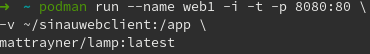
\includegraphics[scale=1]{1.png}\\
    \caption{Menjalankan server}
\end{minipage}
\begin{minipage}{\linewidth}
    \centering
    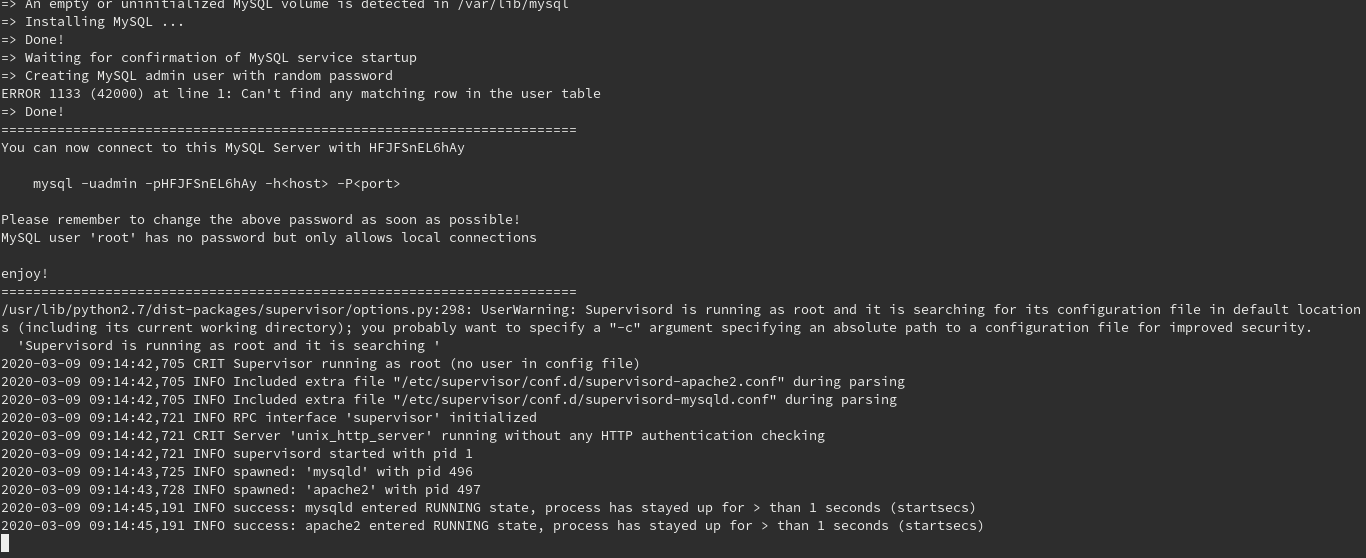
\includegraphics[scale=.3]{2.png}\\
    \caption{Output server}
\end{minipage}\\[2ex]

Kemudian edit file index.php dari pertemuan 5.
\begin{lstlisting}[style=PHP]
<!DOCTYPE html>
<html>

<head>
    <link rel="stylesheet" href="css/style.css" />
</head>

<body>
    <div class="container">
        <div class="main">
            <form method="GET" action="proses.php" id="form">
                <h2>DATA IDENTITAS</h2>
                <hr />
                <label>Nama :</label>
                <input type="text" name="fnama" id="fnama" />
                <label>Alamat :</label>
                <input type="text" name="lalamat" id="lalamat" />
                <p>
                    <label>Jenis Kelamin : </label>
                    <input type="radio" name="jkel" value="Laki-laki" />Laki-laki
                    <input type="radio" name="jkel" value="Perempuan" />Perempuan
                </p>

                <p>
                    <label> Program Studi </label>
                    <select name="prodi">
                        <option value="SI">SI</option>
                        <option value="TI">TI</option>
                        <option value="TK">TK</option>
                        <option value="KA">KA</option>
                        <option value="MI">MI</option>
                    </select>
                </p>

                <p>
                    <label>Hobi</label>
                    <input type="checkbox" name="cekhobi[]" value="Menyanyi" />
                    <label for="chkSing">Menyanyi</label>
                    <input type="checkbox" name="cekhobi[]" value="olah raga" />
                    <label for="cekhobi">Olah Raga</label>
                </p>
                <input type="submit" name="submit" id="submit" value="submit">
            </form>
            <?php include "proses.php"; ?>
        </div>
    </div>
</body>

</html>
\end{lstlisting}

File index.php, pada baris code \lstinline{action="index.php"} dirubah menjadi \lstinline{action="proses.php"}. Kemudian
baris code \lstinline{<?php include "proses.php";?>} dihapus.\\

Setelah itu buat label Jenis Kelamin untuk melabeli tag radio kita. Untuk membuat checkbox radio, gunakan tag
\lstinline{input type="radio"/>. Tag input type radio berfungsi untuk membuat tombol radio atau tombol pilihan
yang diisi dengan cara memilih dari salah satu tombol radio yang ada. Radio biasa
digunakan untuk pilihan yang membatasi user untuk memilih satu dari pilihan yang ada.\\

Setelah itu, kita buat Select. Tag select di dalam HTML digunakan untuk membuat objek form yang berupa list
pilihan yang dapat dipilih oleh user. Biasanya tag select digunakan untuk “memaksa”
user memilih salah satu dari pilihan yang tersedia. Pilihan ini telah didefenisikan pada
saat form dibuat.\\

Lalu buat checkbox dengan elemen checkbox. Tag Input type checkbox berfungsi untuk membuat checkbox atau kotak isian yang
diisi dengan cara menceklist kotak tersebut. checkbox biasa digunakan untuk pilihan
yang dapat dipilih dengan lebih dari 1 pilihan.

\subsubsection{Praktik 2}
Modifikasi file proses.php dari pertemuan 5.
\begin{lstlisting}[style=PHP]
<?php
if (isset($_POST['fnama'])) {
    $fnama = $_POST['fnama'];
    $lalamat = $_POST['lalamat'];
    $jkel=$_POST['jkel'];
    $prodi=$_POST['prodi'];
    echo "<span class='success'>Dengan <b>METODE POST</b></span><br/>";
    echo "Nama : " . $fnama . "<br/>";
    echo "Alamat : " . $lalamat . "<br/>";
    echo "Jenis Kelamin : " . $jkel . "<br/>";
    echo "Program Studi : " . $prodi . "<br/>";

    echo "hobi:<br/> ";
    if(!empty($_POST['cekhobi'])){
        foreach($_POST['cekhobi'] as $selected) {
            echo $selected."</br>";
        }
    }
}
\end{lstlisting}
Modifikasi bagian POST. Pada file proses.php tersebut ditambahkan variabel sesuai yang dengan kita tambahkan tadi pada
bagian file index.php. Untuk menampilkan nilai dari variabel yang nilainya sudah dimasukkan gunakan echo.

\begin{minipage}{\linewidth}
    \centering
    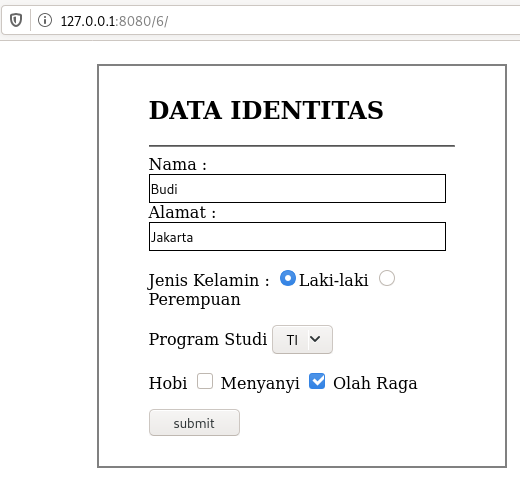
\includegraphics[scale=.5]{index.png}\\
    \caption{Tampilan form}
\end{minipage}
\begin{minipage}{\linewidth}
    \centering
    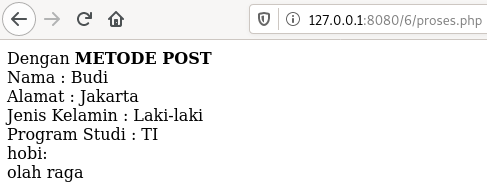
\includegraphics[scale=.6]{post.png}\\
    \caption{Tampilan setelah submit}
\end{minipage}

\subsection{Latihan}
Menerapkan penerimaan input pada metode get
\begin{lstlisting}[style=PHP]
<?php
if (isset($_POST['fnama'])) {
    $fnama = $_POST['fnama'];
    $lalamat = $_POST['lalamat'];
    $jkel=$_POST['jkel'];
    $prodi=$_POST['prodi'];
    echo "<span class='success'>Dengan <b>METODE POST</b></span><br/>";
    echo "Nama : " . $fnama . "<br/>";
    echo "Alamat : " . $lalamat . "<br/>";
    echo "Jenis Kelamin : " . $jkel . "<br/>";
    echo "Program Studi : " . $prodi . "<br/>";

    echo "hobi:<br/> ";
    if(!empty($_POST['cekhobi'])){
        foreach($_POST['cekhobi'] as $selected) {
            echo $selected."</br>";
        }
    }
}
//------------------------------------------------------
if (isset($_GET['fnama'])) {
    $fnama = $_GET['fnama'];
    $lalamat = $_GET['lalamat'];
    $jkel=$_GET['jkel'];
    $prodi=$_GET['prodi'];
    echo "<span class='success'>Dengan <b>METODE GET</b></span><br/>";
    echo "Nama : " . $fnama . "<br/>";
    echo "Alamat : " . $lalamat . "<br/>";
    echo "Jenis Kelamin : " . $jkel . "<br/>";
    echo "Program Studi : " . $prodi . "<br/>";

    echo "hobi:<br/> ";
    if(!empty($_GET['cekhobi'])){
        foreach($_GET['cekhobi'] as $selected) {
            echo $selected."</br>";
        }
    }
}
\end{lstlisting}
Untuk menerapkan input pada metode get, gita hanya perlu mengganti POST pada file proses.php menjadi GET.\\
\begin{minipage}{\linewidth}
    \centering
    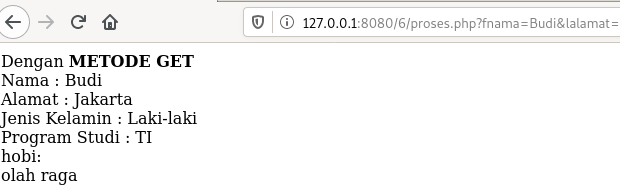
\includegraphics[scale=.6]{get.png}\\
    \caption{Tampilan setelah submit}
\end{minipage}

\newpage

\subsection{Tugas}
Menambahkan input komentar
\begin{lstlisting}[style=PHP]
<p>
    <textarea></textarea>
</p>
\end{lstlisting}
Untuk menampahakn kolom komentar pada input, tambahkan kode tersebut didalam elemen form. Objek form textarea digunakan
untuk membuat text inputan yang bisa menampung lebih dari 1 baris inputan. Tag textarea mirip dengan tag input type
text, namun memiliki kelebihan untuk menampung beberapa baris.\\
\begin{minipage}{\linewidth}
    \centering
    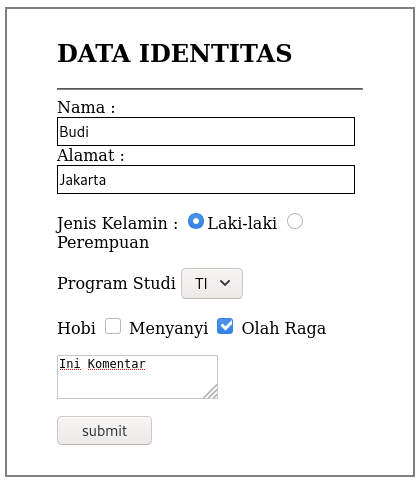
\includegraphics[scale=.8]{komen.png}\\
    \caption{Tampilan setelah ditambah input komentar}
\end{minipage}

\newpage

\section{Kesimpulan}
Setelah praktik ini mahasiswa mampu menuliskan script HTML untuk element-element Form.

\end{document}
